\documentclass{beamer}
\usetheme{Dresden}
\usefonttheme[onlymath]{serif}

\usepackage{amsmath}
\usepackage{graphicx}
\usepackage{xcolor}
\usepackage{adjustbox}
\usepackage{fontawesome}
\usepackage{tikz}
	\usetikzlibrary{patterns,shapes,arrows,calc,datavisualization.formats.functions,decorations.pathreplacing}
\usepackage{hologo}
\usepackage{showexpl}
\usepackage{hyperref}
\usepackage{calc}
\usepackage{fp}



% This creates a fancy/proper TikZ logo in the text.
\newcommand{\TikZ}{Ti\textit{k}Z~{}}





% This defines the way we render the code blocks in the slides.  Some modifications from the standard
% are made to make things easier to read when blown up for size.
\lstloadlanguages{[LaTeX]Tex} 
\lstset{ 
	backgroundcolor=\color{white},   % choose the background color; you must add \usepackage{color} or \usepackage{xcolor}; should come as last argument
	basicstyle=\ttfamily\scriptsize,        % the size of the fonts that are used for the code
	breakatwhitespace=false,         % sets if automatic breaks should only happen at whitespace
	breaklines=true,                 % sets automatic line breaking
	captionpos=t,                    % sets the caption-position to top
	commentstyle=\color{green},    % comment style
	deletekeywords={...},            % if you want to delete keywords from the given language
	escapeinside={\%*}{*)},          % if you want to add LaTeX within your code
	extendedchars=true,              % lets you use non-ASCII characters; for 8-bits encodings only, does not work with UTF-8
	firstnumber=0,                   % start line enumeration with line 1000
	frame=single,	                 % adds a frame around the code
	gobble=6,                        % We gobble the first x characters (removes excess tabs)
	keepspaces=true,                 % keeps spaces in text, useful for keeping indentation of code (possibly needs columns=flexible)
	keywordstyle=\color{blue},      % keyword style
	language=[LaTeX]{TeX},                 % the language of the code
	morekeywords={*,...},            % if you want to add more keywords to the set
	numbers=left,                    % where to put the line-numbers; possible values are (none, left, right)
	numbersep=5pt,                   % how far the line-numbers are from the code
	numberstyle=\tiny\color{gray}, % the style that is used for the line-numbers
	rulecolor=\color{black},         % if not set, the frame-color may be changed on line-breaks within not-black text (e.g. comments (green here))
	showspaces=false,                % show spaces everywhere adding particular underscores; it overrides 'showstringspaces'
	showstringspaces=false,          % underline spaces within strings only
	showtabs=false,                  % show tabs within strings adding particular underscores
	stepnumber=2,                    % the step between two line-numbers. If it's 1, each line will be numbered
	stringstyle=\color{mauve},     % string literal style
	tabsize=2,	                   % sets default tabsize to 2 spaces
	title=\lstname                   % show the filename of files included with \lstinputlisting; also try caption instead of title
}




% This is the title card info.
\title{An Introduction to \TikZ}

%\thanks{\href{https://github.com/BlueNalgene/Introduction_to_LaTeX}{https://github.com/BlueNalgene/Introduction\_to\_LaTeX}}
\author{Wesley T. Honeycutt}
\institute{University of Oklahoma}
\date{\today}





% Here, I create custom colors to match the OU style, and apply it to the Beamer layout
\definecolor{OUCrimson}{RGB}{132 22 23} % UBC Blue (primary)
\definecolor{OUCream}{RGB}{253 249 216} % UBC Grey (secondary)

\setbeamercolor{palette primary}{bg=OUCrimson,fg=white}
\setbeamercolor{palette secondary}{bg=OUCrimson,fg=white}
\setbeamercolor{palette tertiary}{bg=OUCrimson,fg=white}
\setbeamercolor{palette quaternary}{bg=OUCrimson,fg=white}
\setbeamercolor{structure}{fg=OUCrimson} % itemize, enumerate, etc
\setbeamercolor{section in toc}{fg=OUCrimson} % TOC sections

% Override palette coloring with secondary
\setbeamercolor{subsection in head/foot}{bg=OUCream,fg=white}






% I customized the href code so that the links stand out during presentations.
\makeatletter
\Hy@AtBeginDocument{%
	\def\@pdfborder{0 0 1}% Overrides border definition set with colorlinks=true
	\def\@pdfborderstyle{0 0 0}% Overrides border style set with colorlinks=true
	% Hyperlink border style will be underline of width 1pt
}
\makeatother
\hypersetup{%
	colorlinks=true,% hyperlinks will have color
	linkcolor=blue,
	urlcolor=blue,
	linkbordercolor=blue,% hyperlink borders will be red
	pdfborderstyle={/S/U/W 0}% border style will be underline of width 1pt
}






% These are custom defines for the MOSFET example
\newcommand{\metalone}{[pattern= horizontal lines, pattern color=blue]}
\newcommand{\metaltwo}{[pattern= vertical lines, pattern color=purple]}
\newcommand{\poly}{[pattern= grid, pattern color=red]}
\newcommand{\pdiff}{[pattern= north east lines, pattern color=orange]}
\newcommand{\ndiff}{[pattern= north west lines, pattern color=green]}
\newcommand{\pwell}{[pattern= crosshatch dots, pattern color=orange]}
\newcommand{\nwell}{[pattern= crosshatch dots, pattern color=green]}
\newcommand{\oxide}{[pattern = bricks, pattern color = olive]}
\newcommand{\silicon}{[fill = white]}
\newcommand{\metalthree}{[fill = teal]}





\graphicspath{ {images/} } %this removes clutter from the root folder




\begin{document}

	\frame{\titlepage
			\footnotetext{\href{https://github.com/BlueNalgene/Tikz_in_an_hour}{https://github.com/BlueNalgene/Tikz\_in\_an\_hour}}
		}
	
	\frame{\tableofcontents}
	
	\section{Sources and Background}
	
		\frame{\frametitle{What Are We Doing Here?}
			
			\begin{itemize}
				\item<1-> This workshop assumes you have some \LaTeX competency.
				\item<2-> You can code along with a computer using your favorite editor.  Overleaf will be used for examples.
				\item<3-> This workshop covers concepts, full lists of tools are available online:
				\begin{itemize}
					\item<3-> \href{https://pgf-tikz.github.io/pgf/pgfmanual.pdf}{The Official Manual}
					\item<3-> \href{https://cremeronline.com/LaTeX/minimaltikz.pdf}{A Very Minimal Iintroduction to \TikZ}
					\item<3-> \href{https://www.overleaf.com/learn/latex/TikZ_package}{Overleaf's \TikZ Manual}
					\item<3-> \href{https://en.wikibooks.org/wiki/LaTeX/PGF/TikZ}{The \TikZ Wikibook}
				\end{itemize}
			\end{itemize}
		}

		
		\frame{\frametitle{\TikZ Background}
			\begin{itemize}
				\item<1-> \TikZ is a language to control PGF (Portable Graphics Format).
				\item<2-> \TikZ is an acronym for "\TikZ ist \textit{kein} Zeichenprogramm".
				\item<3-> \TikZ is interpreted by \TeX derivative compilers and some graphics programs.
				\item<4-> Lazy people (like me) can export \TikZ code directly from many programs (e.g. Inkscape, Blender, Python, Gnuplot, R)
			\end{itemize}
		}
	
	
	\section{The Environment}
	
		\begin{frame}[fragile]\frametitle{Summon TikZ Environment}
			The \TikZ framework is contained in the \texttt{tikz} package.
			\\~\\
			\only<1>{~\\}
			\only<2>{\TikZ is called using the \texttt{tikzpicture} environment in \LaTeX \\}
			~\\
			The minimum for this environment would be:
			\begin{onlyenv}<1>
				\begin{block}{}
					\begin{lstlisting}
			\documentclass{minimal}
			\usepackage{tikz}
			\begin{document}
				content
			\end{document}
					\end{lstlisting}
				\end{block}
			\end{onlyenv}
			\begin{onlyenv}<2>
				\begin{block}{}
					\begin{lstlisting}
			\documentclass{minimal}
			\usepackage{tikz}
			\begin{document}
				\begin{tikzpicture}
					tikz content
				\end{tikzpicture}
			\end{document}
					\end{lstlisting}
				\end{block}
			\end{onlyenv}
		\end{frame}
	
		\begin{frame}[fragile]\frametitle{Controlling the Environment}
			The \texttt{tikzpicture} environment is controlled like other \LaTeX{} frames.
			
			\begin{lstlisting}
			\documentclass{article}
			\usepackage{tikz}
			\begin{document}
				\begin{figure}[t]
					\centering
					\begin{tikzpicture}
						content here
					\end{tikzpicture}
					\caption{Info about picture}
					\label{fig:my_label}
				\end{figure}
			\end{document}
			\end{lstlisting}
		\end{frame}
	
		\begin{frame}[fragile]\frametitle{Controlling the \textit{Picture}}
			The \texttt{tikzpicture} size should be controlled directly.
		
			\begin{lstlisting}
			\documentclass{article}
			\usepackage{tikz}
			\begin{document}
				\begin{tikzpicture}[scale=3]
					content here
				\end{tikzpicture}
				\\~\\
				\begin{tikzpicture}[xscale=3, yscale=2]
					more content here
				\end{tikzpicture}
			\end{document}
			\end{lstlisting}
	\end{frame}

	
	
	\section{Basic Tools}

	
		\frame{\frametitle{The Basics of The Basics}
			\begin{itemize}
				\item<1-> \TikZ is high level abstraction of vector art commands
				\item<2-> \TikZ is 2D
				\item<3-> 2D Vector = points, curves, and simple operations
				\item<4-> Size matters, reference doesn't
				\item<5-> \TikZ is ridiculously powerful.  The manual is 1000+ pages for a reason.
			\end{itemize}
		}
	
		\frame[containsverbatim]{\frametitle{The General Case}
			
			\begin{lstlisting}
			\command[options, options, options] node connection;
			\end{lstlisting}
			
			\begin{itemize}
				\item<1-> {Within a \TikZ picture environment, each part of a drawing gets a semicolon (;) terminated line.}
				\item<2-> {Optional arguments are contained within square brackets ([, ])}
				\item<3-> {Nodes are the draw point of an object, using Cartesian (x, y) notation.}
				\item<4-> {You may connect nodes with a connection command}
			\end{itemize}
			
		
		}
	
		\frame[containsverbatim]{\frametitle{Arbitrary Reference 1}
			\begin{columns}
				\begin{column}{0.75\textwidth}
					\begin{lstlisting}
			
\begin{tikzpicture}
				\draw (0,0) -- (0,1) -- (1,1) -- cycle;
			\end{tikzpicture}
					\end{lstlisting}
				\end{column}
				\begin{column}{0.25\textwidth}
					
\begin{tikzpicture}
						\draw (0,0) -- (0,1) -- (1,1) -- cycle;
					\end{tikzpicture}
				\end{column}
			\end{columns}
		}
	
		\frame[containsverbatim]{\frametitle{Arbitrary Reference 11}
			\begin{columns}
				\begin{column}{0.75\textwidth}
					\begin{lstlisting}
			
\begin{tikzpicture}
				\draw (10,10) -- (10,11) -- (11,11) -- cycle;
			\end{tikzpicture}
					\end{lstlisting}
				\end{column}
				\begin{column}{0.25\textwidth}
					
\begin{tikzpicture}
						\draw (10,10) -- (10,11) -- (11,11) -- cycle;
					\end{tikzpicture}
				\end{column}
			\end{columns}
		}

		\frame[containsverbatim]{\frametitle{Size and Reference}
			\begin{columns}
				\begin{column}{0.75\textwidth}
					\begin{lstlisting}
			\begin{tikzpicture}
				\draw (0,10) -- (0,10) -- (10,10) -- cycle;
			\end{tikzpicture}
					\end{lstlisting}
				\end{column}
				\begin{column}{0.25\textwidth}
					\begin{tikzpicture}
						\draw (0,0) -- (0,10) -- (10,10) -- cycle;
					\end{tikzpicture}
				\end{column}
			\end{columns}
		}
	
		\frame[containsverbatim]{\frametitle{Default Unit = 1cm}
			\begin{columns}
				\begin{column}{0.75\textwidth}
					\begin{lstlisting}
			
\begin{tikzpicture}[x=1cm,y=2cm]
				\draw (0,0) -- (0,1) -- (1,1) -- cycle;
			\end{tikzpicture}
					\end{lstlisting}
				\end{column}
				\begin{column}{0.25\textwidth}
					
\begin{tikzpicture}[x=1cm,y=2cm]
						\draw (0,0) -- (0,1) -- (1,1) -- cycle;
					\end{tikzpicture}
				\end{column}
			\end{columns}
		}
	
		\frame[containsverbatim]{\frametitle{Drawings are Altered When Called by \textit{\\draw}}
			\begin{block}{}
				\begin{lstlisting}
			
\begin{tikzpicture}
				\draw[red, very thick, rounded corners=9pt] (0,0) -- (0,1) -- (1,1) -- cycle;
			\end{tikzpicture}
				\end{lstlisting}
			\end{block}
			\begin{center}
				
\begin{tikzpicture}
					\draw[red, very thick, rounded corners=9pt] (0,0) -- (0,1) -- (1,1) -- cycle;
				\end{tikzpicture}
			\end{center}
		}
	
		\frame[containsverbatim]{\frametitle{Altering Connections with Circles}
			\begin{lstlisting}
			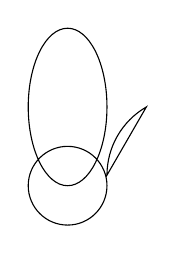
\begin{tikzpicture}
				\draw (0,0) circle [radius=.5cm] (0,1) circle [x radius=.5cm, y radius=1cm] (1,1) arc (120:180:1) -- cycle;
			\end{tikzpicture}
			\end{lstlisting}
		
			\begin{center}
				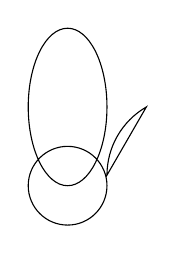
\begin{tikzpicture}
					\draw (0,0) circle [radius=.5cm] (0,1) circle [x radius=.5cm, y radius=1cm] (1,1) arc (120:180:1) -- cycle;
				\end{tikzpicture}
			\end{center}
		}
	
		\frame[containsverbatim]{\frametitle{How did those Arcs work?}
			\begin{lstlisting}
			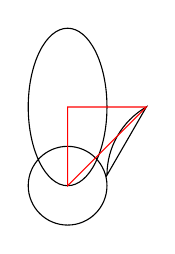
\begin{tikzpicture}
				\draw (0,0) circle [radius=.5cm] (0,1) circle [x radius=.5cm, y radius=1cm] (1,1) arc (120:180:1) -- cycle;
				\draw[red] (0,0) -- (0,1) -- (1,1) -- cycle;
			\end{tikzpicture}
			\end{lstlisting}
			
			\begin{center}
				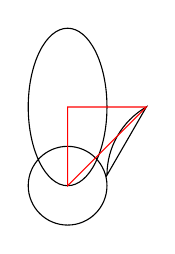
\begin{tikzpicture}
					\draw (0,0) circle [radius=.5cm] (0,1) circle [x radius=.5cm, y radius=1cm] (1,1) arc (120:180:1) -- cycle;
					\draw[red] (0,0) -- (0,1) -- (1,1) -- cycle;
				\end{tikzpicture}
			\end{center}
		}
		
		
		\frame[containsverbatim]{\frametitle{Grids with Defined Steps}
			\begin{lstlisting}
			
\begin{tikzpicture}
				\draw[step=.5cm, gray, very thin] (-1.2,-1.2) grid (1.2,1.2);
			\end{tikzpicture}
			\end{lstlisting}
			
			\begin{center}
				
\begin{tikzpicture}
					\draw[step=.5cm, gray, very thin] (-1.2,-1.2) grid (1.2,1.2);
				\end{tikzpicture}
			\end{center}
		}
		
		\frame[containsverbatim]{\frametitle{Coordinate Labels, Simple Arrows}
			\begin{lstlisting}
			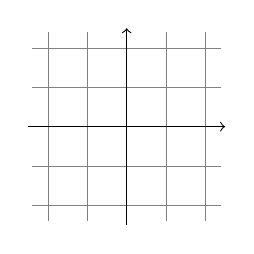
\begin{tikzpicture}
				\draw[step=.5cm, gray, very thin] (-1.2,-1.2) grid (1.2,1.2);
				\draw[->] (-1.25,0) -- (1.25,0) coordinate (x axis);
				\draw[->] (0,-1.25) -- (0,1.25) coordinate (y axis);
			\end{tikzpicture}
			\end{lstlisting}
			
			\begin{center}
				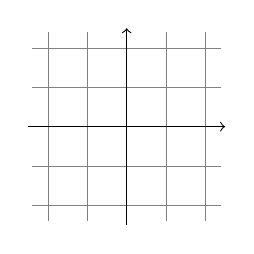
\begin{tikzpicture}
					\draw[step=.5cm, gray, very thin] (-1.2,-1.2) grid (1.2,1.2);
					\draw[->] (-1.25,0) -- (1.25,0) coordinate (x axis);
					\draw[->] (0,-1.25) -- (0,1.25) coordinate (y axis);
				\end{tikzpicture}
			\end{center}
		}
		
		\frame[containsverbatim]{\frametitle{Right Angle Connections, Using Coordinate Labels}
			\begin{lstlisting}
			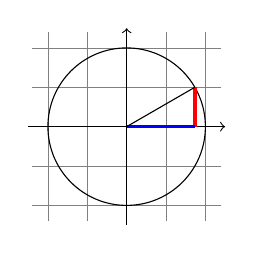
\begin{tikzpicture}
				\draw[step=.5cm, gray, very thin] (-1.2,-1.2) grid (1.2,1.2);
				\draw[->] (-1.25,0) -- (1.25,0) coordinate (x axis);
				\draw[->] (0,-1.25) -- (0,1.25) coordinate (y axis);
				\draw (0,0) circle (1cm);
				\draw[very thick,red] (30:1cm) --  (30:1cm |- x axis);
				\draw[very thick,blue] (30:1cm |- x axis) -- (0,0);
				\draw (0,0) -- (30:1cm);
			\end{tikzpicture}
			\end{lstlisting}
			
			\begin{center}
				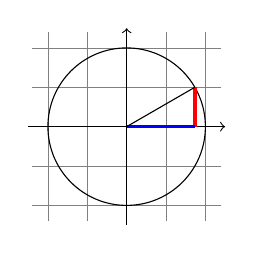
\begin{tikzpicture}
					\draw[step=.5cm, gray, very thin] (-1.2,-1.2) grid (1.2,1.2);
					\draw[->] (-1.25,0) -- (1.25,0) coordinate (x axis);
					\draw[->] (0,-1.25) -- (0,1.25) coordinate (y axis);
					\draw (0,0) circle (1cm);
					\draw[very thick,red] (30:1cm) -- (30:1cm |- x axis);
					\draw[very thick,blue] (30:1cm |- x axis) -- (0,0);
					\draw (0,0) -- (30:1cm);
				\end{tikzpicture}
			\end{center}
		}
	
	
		\frame[containsverbatim]{\frametitle{Nodes as Text Labels}
			\begin{block}{Node Syntax:}
				\texttt{node{[}}\textit{anchor, options}\texttt{{]} \{}\textit{contents}\texttt{\}}
			\end{block}
			\begin{lstlisting}
			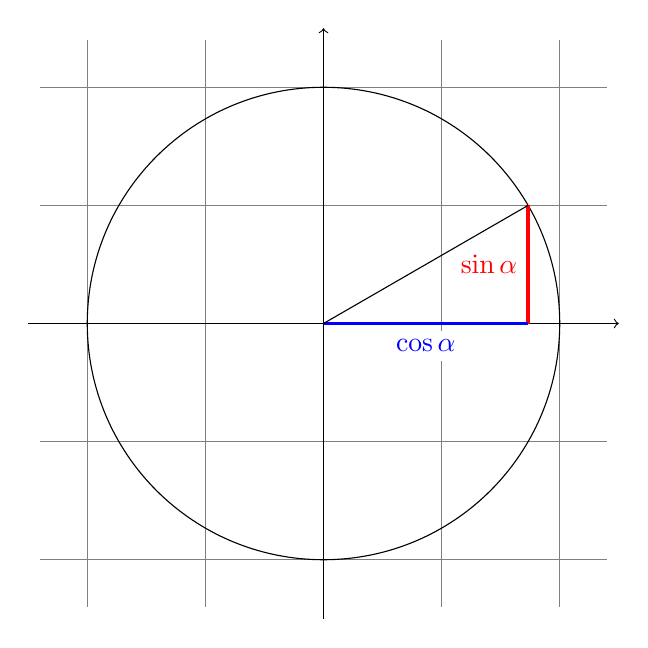
\begin{tikzpicture}[scale=3]
				\draw[step=.5cm, gray, very thin] (-1.2,-1.2) grid (1.2,1.2);
				\draw[->] (-1.25,0) -- (1.25,0) coordinate (x axis);
				\draw[->] (0,-1.25) -- (0,1.25) coordinate (y axis);
				\draw (0,0) circle (1cm);
				\draw[very thick,red] (30:1cm) -- node[left,fill=white] {$\sin \alpha$} (30:1cm |- x axis);
				\draw[very thick,blue] (30:1cm |- x axis) -- node[below=2pt,fill=white] {$\cos \alpha$} (0,0);
				\draw (0,0) -- (30:1cm);
			\end{tikzpicture}
			\end{lstlisting}
		}
	
		\frame{\frametitle{Nodes as Text Labels - Result}
			\begin{center}
				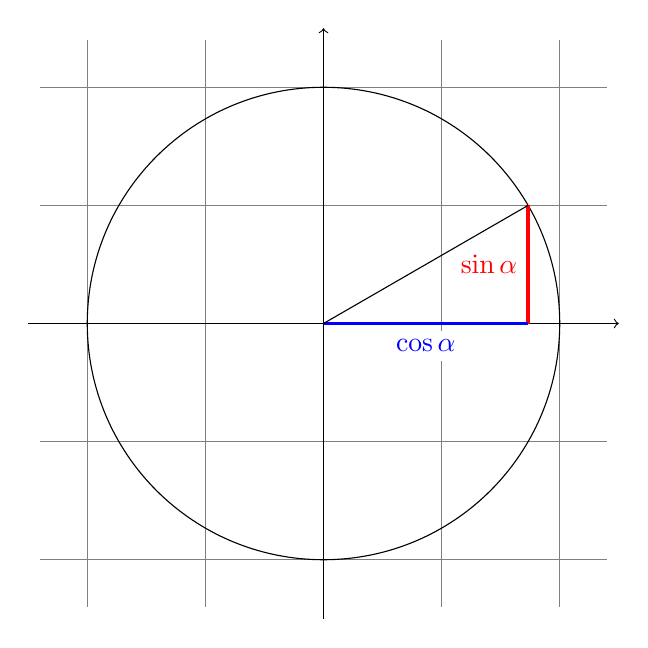
\begin{tikzpicture}[scale=3]
					\draw[step=.5cm, gray, very thin] (-1.2,-1.2) grid (1.2,1.2);
					\draw[->] (-1.25,0) -- (1.25,0) coordinate (x axis);
					\draw[->] (0,-1.25) -- (0,1.25) coordinate (y axis);
					\draw (0,0) circle (1cm);
					\draw[very thick,red] (30:1cm) -- node[left,fill=white] {$\sin \alpha$} (30:1cm |- x axis);
					\draw[very thick,blue] (30:1cm |- x axis) -- node[below=2pt,fill=white] {$\cos \alpha$} (0,0);
					\draw (0,0) -- (30:1cm);
				\end{tikzpicture}
			\end{center}
		}
	
		\frame[containsverbatim]{\frametitle{Custom Colors, Filled Areas}
			\begin{lstlisting}
			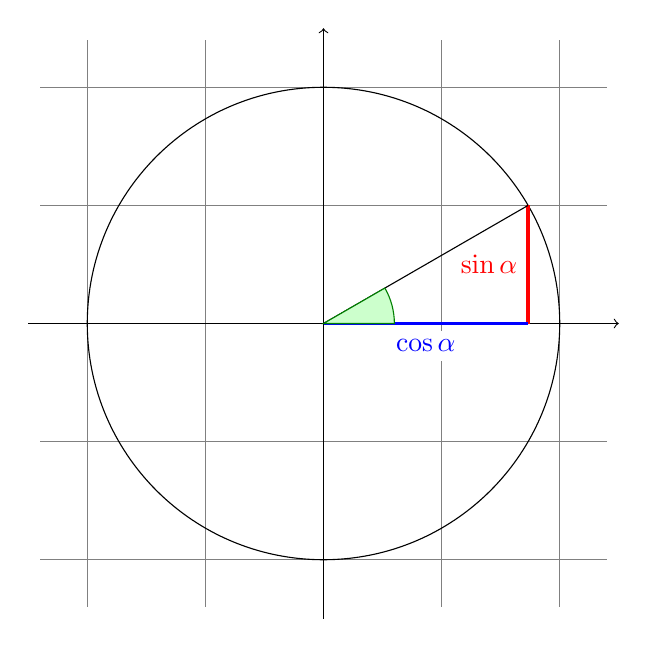
\begin{tikzpicture}[scale=3]
				\draw[step=.5cm, gray, very thin] (-1.2,-1.2) grid (1.2,1.2);
				\draw[->] (-1.25,0) -- (1.25,0) coordinate (x axis);
				\draw[->] (0,-1.25) -- (0,1.25) coordinate (y axis);
				\draw (0,0) circle (1cm);
				\draw[very thick,red] (30:1cm) -- node[left,fill=white] {$\sin \alpha$} (30:1cm |- x axis);
				\draw[very thick,blue] (30:1cm |- x axis) -- node[below=2pt,fill=white] {$\cos \alpha$} (0,0);
				\draw (0,0) -- (30:1cm);
				\filldraw[fill=green!20,draw=green!50!black] (0,0) -- (3mm,0mm) arc (0:30:3mm) -- cycle;
			\end{tikzpicture}
			\end{lstlisting}
		}
	
		\frame{\frametitle{Custom Colors, Filled Areas - Result}
			\begin{center}
				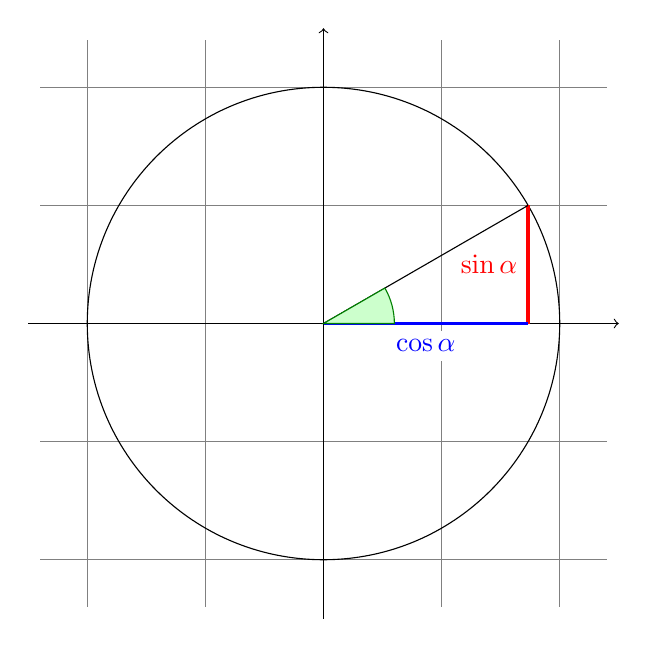
\begin{tikzpicture}[scale=3]
					\draw[step=.5cm, gray, very thin] (-1.2,-1.2) grid (1.2,1.2);
					\draw[->] (-1.25,0) -- (1.25,0) coordinate (x axis);
					\draw[->] (0,-1.25) -- (0,1.25) coordinate (y axis);
					\draw (0,0) circle (1cm);
					\draw[very thick,red] (30:1cm) -- node[left,fill=white] {$\sin \alpha$} (30:1cm |- x axis);
					\draw[very thick,blue] (30:1cm |- x axis) -- node[below=2pt,fill=white] {$\cos \alpha$} (0,0);
					\draw (0,0) -- (30:1cm);
					\filldraw[fill=green!20,draw=green!50!black] (0,0) -- (3mm,0mm) arc (0:30:3mm) -- cycle;
				\end{tikzpicture}
			\end{center}
		}
		
		\frame[containsverbatim]{\frametitle{Loops}
			\begin{lstlisting}
			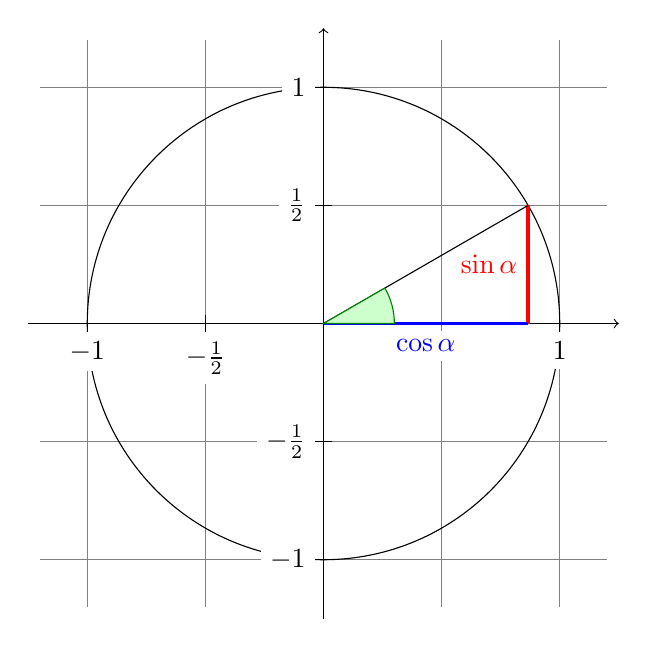
\begin{tikzpicture}[scale=3]
				\draw[step=.5cm, gray, very thin] (-1.2,-1.2) grid (1.2,1.2);
				\draw[->] (-1.25,0) -- (1.25,0) coordinate (x axis);
				\draw[->] (0,-1.25) -- (0,1.25) coordinate (y axis);
				\draw (0,0) circle (1cm);
				\draw[very thick,red] (30:1cm) -- node[left,fill=white] {$\sin \alpha$} (30:1cm |- x axis);
				\draw[very thick,blue] (30:1cm |- x axis) -- node[below=2pt,fill=white] {$\cos \alpha$} (0,0);
				\draw (0,0) -- (30:1cm);
				\filldraw[fill=green!20,draw=green!50!black] (0,0) -- (3mm,0mm) arc (0:30:3mm) -- cycle;
				\foreach \x/\xtext in {-1, -0.5/-\frac{1}{2}, 1} 
				\draw (\x cm,1pt) -- (\x cm,-1pt) node[anchor=north,fill=white] {$\xtext$};
				\foreach \y/\ytext in {-1, -0.5/-\frac{1}{2}, 0.5/\frac{1}{2}, 1} 
				\draw (1pt,\y cm) -- (-1pt,\y cm) node[anchor=east,fill=white] {$\ytext$};
			\end{tikzpicture}
			\end{lstlisting}
		}
	
		\frame[containsverbatim]{\frametitle{Loop - Syntax}
			\begin{block}{\TikZ}
				content...
			\end{block}
			\begin{block}{C}
				\begin{lstlisting}
				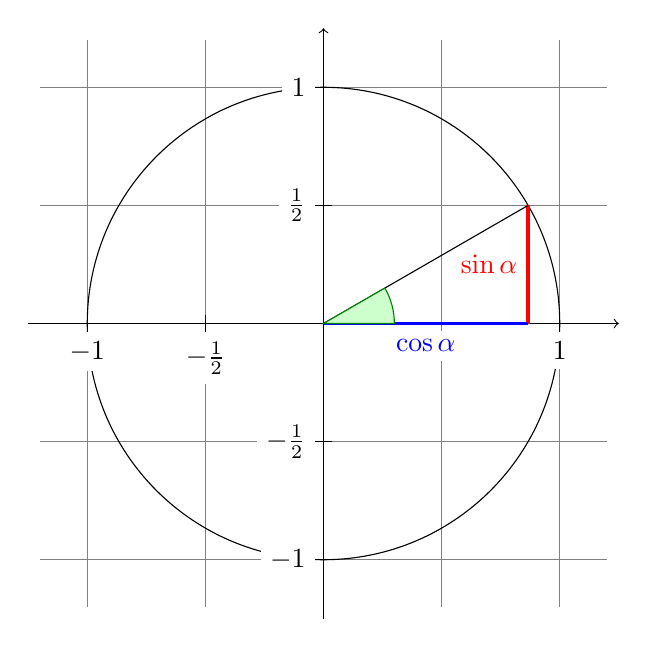
\begin{tikzpicture}[scale=3]
				\draw[step=.5cm, gray, very thin] (-1.2,-1.2) grid (1.2,1.2);
				\draw[->] (-1.25,0) -- (1.25,0) coordinate (x axis);
				\draw[->] (0,-1.25) -- (0,1.25) coordinate (y axis);
				\draw (0,0) circle (1cm);
				\draw[very thick,red] (30:1cm) -- node[left,fill=white] {$\sin \alpha$} (30:1cm |- x axis);
				\draw[very thick,blue] (30:1cm |- x axis) -- node[below=2pt,fill=white] {$\cos \alpha$} (0,0);
				\draw (0,0) -- (30:1cm);
				\filldraw[fill=green!20,draw=green!50!black] (0,0) -- (3mm,0mm) arc (0:30:3mm) -- cycle;
				\foreach \x/\xtext in {-1, -0.5/-\frac{1}{2}, 1} 
				\draw (\x cm,1pt) -- (\x cm,-1pt) node[anchor=north,fill=white] {$\xtext$};
				\foreach \y/\ytext in {-1, -0.5/-\frac{1}{2}, 0.5/\frac{1}{2}, 1} 
				\draw (1pt,\y cm) -- (-1pt,\y cm) node[anchor=east,fill=white] {$\ytext$};
				\end{tikzpicture}
				\end{lstlisting}
			\end{block}
			
		}
		
		\frame{\frametitle{Loops - Result}
%			\vspace{-5pt}
			\begin{center}
				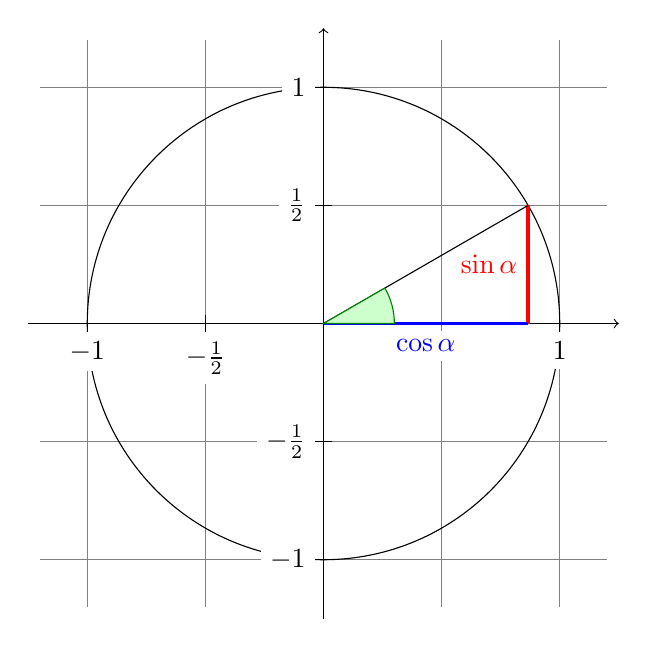
\begin{tikzpicture}[scale=3]
					\draw[step=.5cm, gray, very thin] (-1.2,-1.2) grid (1.2,1.2);
					\draw[->] (-1.25,0) -- (1.25,0) coordinate (x axis);
					\draw[->] (0,-1.25) -- (0,1.25) coordinate (y axis);
					\draw (0,0) circle (1cm);
					\draw[very thick,red] (30:1cm) -- node[left,fill=white] {$\sin \alpha$} (30:1cm |- x axis);
					\draw[very thick,blue] (30:1cm |- x axis) -- node[below=2pt,fill=white] {$\cos \alpha$} (0,0);
					\draw (0,0) -- (30:1cm);
					\filldraw[fill=green!20,draw=green!50!black] (0,0) -- (3mm,0mm) arc (0:30:3mm) -- cycle;
					\foreach \x/\xtext in {-1, -0.5/-\frac{1}{2}, 1} 
					\draw (\x cm,1pt) -- (\x cm,-1pt) node[anchor=north,fill=white] {$\xtext$};
					\foreach \y/\ytext in {-1, -0.5/-\frac{1}{2}, 0.5/\frac{1}{2}, 1} 
					\draw (1pt,\y cm) -- (-1pt,\y cm) node[anchor=east,fill=white] {$\ytext$};
				\end{tikzpicture}
			\end{center}
		}


	\section{Libraries}
	
		\frame[containsverbatim]{\frametitle{Libraries and How to Summon Them}
			\begin{block}{Syntax in Preamble:}
				\begin{lstlisting}
				\usetikzlibrary{library}
				\end{lstlisting}
			\end{block}
		
			\begin{itemize}
				\item I can list all of the libraries with a minimal description, but there will not be time to give examples of each.
				\item I recommend \href{https://tex.stackexchange.com/questions/42611/list-of-available-tikz-libraries-with-a-short-introduction}{this comprehensive Stack Overflow thread} which attempts to provide an introduction for each library with examples.
				\item Official documentation in \href{https://pgf-tikz.github.io/pgf/pgfmanual.pdf}{Part V of the manual}.
			\end{itemize}
		}


		\frame{\frametitle{\TikZ Libraries in Brief (1/6)}
			\begin{block}{How to read this list:}
				\begin{description}
					\item[Descriptive Name] (\texttt{Library command}) - One line description
				\end{description}
			\end{block}
		
			\begin{description}
				\item[Three Dimensions] (\texttt{3D}) - Produce plots using cylindrical or spherical coordinate systems with predefined planes.
				\item[Angles] \texttt{(angle)} - Draw angles between nodes and connections.
				\item[Arrow Tip] \texttt{(arrows.meta)} - Add arrowheads and special dots to your node connections.
				\item[Automata] \texttt{(automata)} - Draw finite automata and Turing machines.
				\item[Babel] \texttt{(babel)} - Helps \TikZ behave better with non-standard characters like \o.
			\end{description}
		}
	
		\frame{\frametitle{\TikZ Libraries in Brief (2/6)}
			\begin{description}
				\item[Backgrounds] \texttt{(background)} - Put a background behind your drawing.
				\item[Calculator] \texttt{(calc)} - Uses \TeX to calculate values.
				\item[Calendar] \texttt{calendar)} - Draw a calendar.
				\item[Chains] \texttt{(chains)} - Enable more complex connection between nodes.
				\item[Circuits] \texttt{(circuits)} - Draw electronic circuits.
				\item[Decorations] \texttt{(decoration)} - Fancy connections like squiggles, zig-zags, text, and shapes.
				\item[Entity-Relationship] \texttt{(er)} - Tools for drawing entity-relationship coded diagrams.
				\item[Externalization] \texttt{(external)} - Semi-automatic export of \TikZ pictures.
			\end{description}
		}
				
				
		\frame{\frametitle{\TikZ Libraries in Brief (3/6)}
			\begin{description}
				\item[Fading] \texttt{(fadings)} - Create gradients between color and transparency.
				\item[Fitting] \texttt{(fit)} - Fit a bounding box or circle around all the nodes you list in the command.
				\item[Fixed Points] \texttt{(fixedpointarithmetic)} - Allow big numbers in calculations.
				\item[Floating Points] \texttt{(fpu)} - Allow precise numbers in calculations.
				\item[Lindenmayer Systems] \texttt{(lindenmayersystems)} - Draw branching and fractal designs.
				\item[Math] \texttt{(math)} - Perform calculations in a user-friendly way.
				\item[Matrix] \texttt{(matrix)} - Draw matrices and operations on them.
				\item[Mindmap] \texttt{(mindmap)} - Draw \textit{mindmap} style relationship trees.
			\end{description}
		}
	

		\frame{\frametitle{\TikZ Libraries in Brief (4/6)}
			\begin{description}	
				\item[Paper Folding] \texttt{(folding)} - Draw objects which may be printed, cut, and then assembled into 3D objects.
				\item[Patterns] \texttt{(patterns])} - Hatches, lines, dots, and other fill patterns.
				\item[Three Point Perspective] \texttt{(perspective)} - Draw with up to 3 vanishing points for a 3D effect.
				\item[Petri-Net] \texttt{(petri)} - Draw Petri-Net style logic diagrams
				\item[Plot Extension] \texttt{(plothandlers)} - Adds even more ways you can use connections (partial lines, splines, gaps)
				\item[Plot Marks] \texttt{(plotmarks)} - More shapes for your nodes.
				\item[Profiler] \texttt{(profiler)} - Debugging tools and timers for compiling.
			\end{description}
		}
		
	
		\frame{\frametitle{\TikZ Libraries in Brief (5/6)}
			\begin{description}
				\item[Resource Description] \texttt{(rdf)} - Output files with more descriptive comments to make them human-readable.
				\item[Shading] \texttt{(shadings)} - Creates color gradients.
				\item[Shadow] \texttt{(shadows)} - Create drop shadows behind nodes and connections.
				\item[Shapes] \texttt{(shapes)} - Add pre-defined common shapes.
				\begin{description}
					\item[Multipart] \texttt{(shapes.multipart)} - Shapes with dividing lines.
					\item[Callouts] \texttt{(shapes.callouts)} - Create callouts (speech bubbles).
					\item[Misc] \texttt{(shapes.misc)} - More pre-defined shapes.
					
				\end{description}
				\item[Spy] \texttt{(spy)} - Spy on or zoom in on part of your drawing like an inset map.
				
			\end{description}
		}
		
	
		\frame{\frametitle{\TikZ Libraries in Brief (6/6)}
			\begin{description}
				\item[SVG Path] \texttt{(svg.path)} - Create your own connection paths using SVG rules.
				\item[To Path] \texttt{(topaths)} - Treat your connections as a ``path'' for vector outputs.
				\item[Through Points] \texttt{(through)} - Make your connections go \emph{through} a node rather than \emph{to} a point.
				\item[Tree] \texttt{(trees)} - Create complex tree connections.
				\item[Turtle Graphics] \texttt{(turtle)} - Draw using ``turtle graphics'' commands rather than pre-defined nodes.
				\item[Views] \texttt{(views)} - Define special rules for the box that contains a TikZ graphic.
			\end{description}
		
		}
	
	\section{Examples}
		
		\frame{\frametitle{Some Practical Examples}
			\begin{block}{You can do nigh-infinite things with \TikZ}
				Here are some examples which touch on useful concepts:
				\begin{itemize}
					\item MOSFET - Using simple nodes to create diagrams.
					\item Amplitude and Frequency
					\item and more...
				\end{itemize}
			\end{block}
		}
	
		
		\frame[containsverbatim]{\frametitle{MOSFET (1/5)}
			We can use the \LaTeX\ definitions to define parts of our drawing in the preamble of our document.
			
			\begin{block}{Custom Colors}
				\begin{lstlisting}
			\newcommand{\metalone}{[pattern= horizontal lines, pattern color=blue]}
				\end{lstlisting}
			\end{block}
		
			For this example, I have defined: \texttt{metalone}, \texttt{metaltwo}, \texttt{metalthree}, \texttt{poly}, \texttt{pdiff}, \texttt{ndiff}, \texttt{pwell}, \texttt{nwell}, \texttt{oxide}, and \texttt{silicon}.
		}
	
		\frame[containsverbatim]{\frametitle{MOSFET (2/5)}
			We can tell connections to make a curve
			
			\begin{block}{Angles In and Out}
				\begin{lstlisting}
			(1,2.5) to [out=270,in=180] (1.5,2)
				\end{lstlisting}
			\end{block}
		}
	
		\frame[containsverbatim]{\frametitle{MOSFET (3/5)}
			We can connect to a node at certain anchor points and add text.
			
			\begin{block}{Anchors and Text}
				\begin{lstlisting}
			(0,.25) node [midway,above] {p doped Si}
				\end{lstlisting}
			\end{block}
		}
		
		
		\frame[containsverbatim]{\frametitle{MOSFET (4/5)}
			
			\begin{lstlisting}[basicstyle=\tiny\tt,]
			\begin{tikzpicture}
			\draw \pdiff (0,.25) -- (0,3) -- (1,3) -- (1,2.5) to [out=270,in=180] (1.5,2) -- (3.75,2) to [out=0,in=270] (4.25,2.5) -- (4.25,3) -- (6.75,3) -- (6.75,2.5) to [out=270,in=180] (7.25,2) -- (9.5,2) to [out=0,in=270] (10,2.5) -- (10,3) -- (11,3) -- (11,.25) -- ;
			\draw \metalthree (0,0) rectangle (11,.25) node [midway, color=white]
			{Si Substrate};
			\draw \oxide (4,3) rectangle (7,4) node [pos=.5,font=\bf\Large] {oxide};
			\draw \metalone (4,4) rectangle (7,4.5);
			\draw \ndiff (4.25,3) -- (1,3) -- (1,2.5) to [out=270,in=180] (1.5,2) -- (3.75,2) to [out=0,in=270] (4.25,2.5) -- (4.25,3) node at (2.625,2.5) [align=center] {n-type};
			\draw \ndiff (10,3) -- (6.75,3) -- (6.75,2.5) to [out=270,in=180] (7.25,2) -- (9.5,2) to [out=0,in=270] (10,2.5) -- (10,3) node at (8.375,2.5) [align=center] {n-type};
			\draw \metalone (1.25,3) rectangle (3,3.5);
			\draw \metalone (8,3) rectangle (9.75,3.5);
			\draw [->] (1,5) node [above] {Source} -- (2.125,3.5);
			\draw [->] (10,5) node [above] {Drain} -- (8.975,3.5);
			\draw [->] (5.5,5) node [above] {Gate} -- (5.5,4.5);
			\node at (5.5,-.5) [align=center] {$V_{GS} < V_{threshold}$};
			\end{tikzpicture}
			\end{lstlisting}
			
		}
	
		\frame{\frametitle{MOSFET (5/5)}
			
			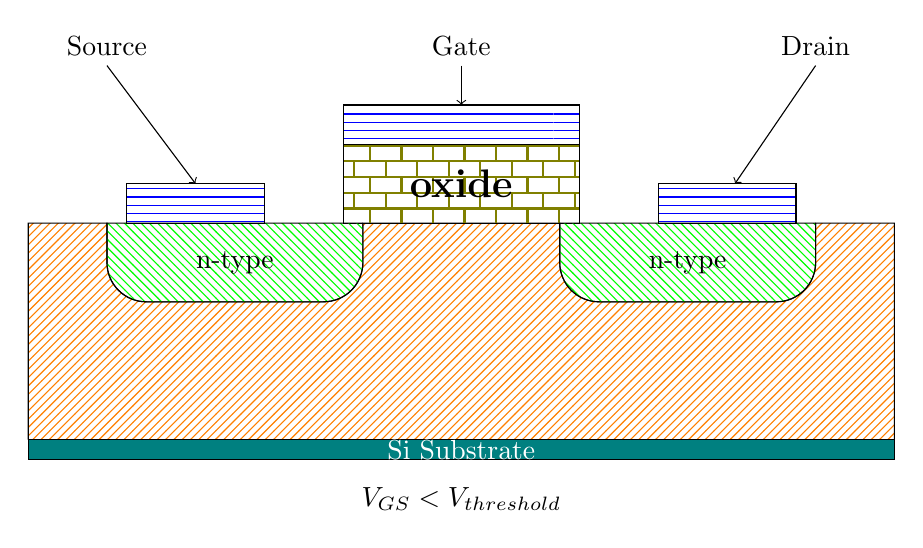
\begin{tikzpicture}
				\draw \pdiff (0,.25) -- (0,3) -- (1,3) -- (1,2.5) to [out=270,in=180] (1.5,2) -- (3.75,2) to [out=0,in=270] (4.25,2.5) -- (4.25,3) -- (6.75,3) -- (6.75,2.5) to [out=270,in=180] (7.25,2) -- (9.5,2) to [out=0,in=270] (10,2.5) -- (10,3) -- (11,3) -- (11,.25) -- (0,.25);
				\draw \metalthree (0,0) rectangle (11,.25) node [midway, color=white]
				{Si Substrate};
				\draw \oxide (4,3) rectangle (7,4) node [pos=.5,font=\bfseries\Large] {oxide};
				\draw \metalone (4,4) rectangle (7,4.5);
				\draw \ndiff (4.25,3) -- (1,3) -- (1,2.5) to [out=270,in=180] (1.5,2) -- (3.75,2) to [out=0,in=270] (4.25,2.5) -- (4.25,3) node at (2.625,2.5) [align=center] {n-type};
				\draw \ndiff (10,3) -- (6.75,3) -- (6.75,2.5) to [out=270,in=180] (7.25,2) -- (9.5,2) to [out=0,in=270] (10,2.5) -- (10,3) node at (8.375,2.5) [align=center] {n-type};
				\draw \metalone (1.25,3) rectangle (3,3.5);
				\draw \metalone (8,3) rectangle (9.75,3.5);
				\draw [->] (1,5) node [above] {Source} -- (2.125,3.5);
				\draw [->] (10,5) node [above] {Drain} -- (8.975,3.5);
				\draw [->] (5.5,5) node [above] {Gate} -- (5.5,4.5);
				\node at (5.5,-.5) [align=center] {$V_{GS} < V_{threshold}$};
			\end{tikzpicture}
			
		}
	
	\frame[containsverbatim]{\frametitle{Amplitude and Frequency (1/5)}
		Let's change course and render a plot to show how amplitude and period of a trigonometric function is altered:
		\begin{equation*}
			f\left(x\right) = A*(\sin{\left(B*\theta\right)})
		\end{equation*}
		We will use a new library:
		\begin{lstlisting}
			\usetikzlibrary{datavisualization.formats.functions}
		\end{lstlisting}

	}

	\frame[containsverbatim]{\frametitle{Amplitude and Frequency (2/5)}
		\begin{columns}
			\begin{column}{0.5\textwidth}
				\begin{itemize}
					\item We first call Data Visualization.
					\item We describe the appearance of the plot (axes, grids).
					\item We describe the lines (smooth, colors, dashes).
					\item We add legend entries for each plot.
					\item Finally, we tell it to expect functions.
				\end{itemize}
			\end{column}
			\begin{column}{0.5\textwidth}
				\begin{lstlisting}[basicstyle=\tiny\tt,]
			\begin{tikzpicture}
			\datavisualization [
			school book axes,
			y axis=grid,
			x axis=grid,
			visualize as smooth line/.list={sina,sinb,sinc},
			style sheet=strong colors,
			style sheet=vary dashing,
			sina={label in legend={text=$\sin x$}},
			sinb={label in legend={text=$ 3 \times{\sin x}$}},
			sinc={label in legend={text=$\sin{\left(3\times x \right)}$}},
			data/format=function]
				\end{lstlisting}
			\end{column}
		\end{columns}
	}

	\frame[containsverbatim]{\frametitle{Amplitude and Frequency (3/5)}
		\begin{columns}
			\begin{column}{0.5\textwidth}
				\begin{itemize}
					\item Each function gets a \texttt{data} entry with a \texttt{set} label.
					\item Variables are defined in an \texttt{interval}.
					\item Functions are defined with \texttt{func}.
					\item Since we are using radians, we have to tell it \texttt{r}.
				\end{itemize}
			\end{column}
			\begin{column}{0.5\textwidth}
				\begin{lstlisting}[basicstyle=\tiny\tt,]
			data [set=sina] {
			var x : interval [-0.5*pi:2*pi];
			func y = sin(\value x r);
			}
			data [set=sinb] {
			var x : interval [-0.5*pi:2*pi];
			func y = 3 * sin(\value x r);
			}
			data [set=sinc] {
			var x : interval [-0.5*pi:2*pi];
			func y = sin(3 * \value x r);
			};
			\end{tikzpicture}
				\end{lstlisting}
			\end{column}
		\end{columns}
		
	}

	\frame{\frametitle{Amplitude and Frequency (4/5)}
		Our complete plot:
		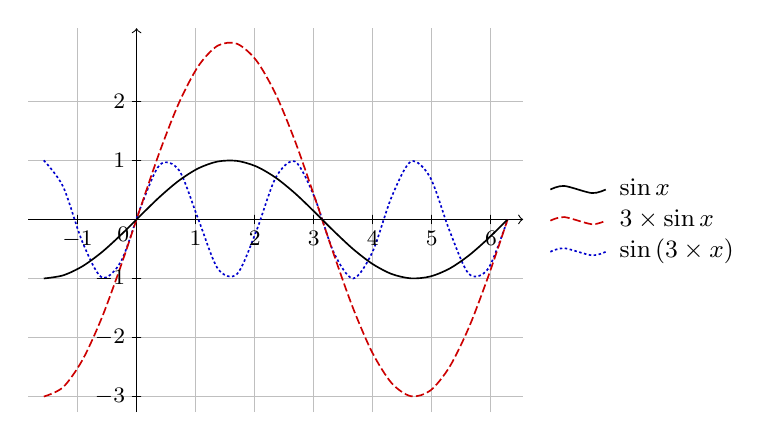
\begin{tikzpicture}[scale=.75]
			\datavisualization [
			school book axes,
			y axis=grid,
			x axis=grid,
			visualize as smooth line/.list={sina,sinb,sinc},
			style sheet=strong colors,
			style sheet=vary dashing,
			sina={label in legend={text=$\sin x$}},
			sinb={label in legend={text=$3\times{\sin x}$}},
			sinc={label in legend={text=$\sin{\left( 3 \times x \right)}$}},
			data/format=function ]
			data [set=sina] {
				var x : interval [-0.5*pi:2*pi];
				func y = sin(\value x r);
			}
			data [set=sinb] {
				var x : interval [-0.5*pi:2*pi];
				func y = 3 * sin(\value x r);
			}
			data [set=sinc] {
				var x : interval [-0.5*pi:2*pi];
				func y = sin(3 * \value x r);
			};
		\end{tikzpicture}
		
	}

	\frame[containsverbatim]{\frametitle{Amplitude and Frequency (5/5)}
		We can add nodes like before:
		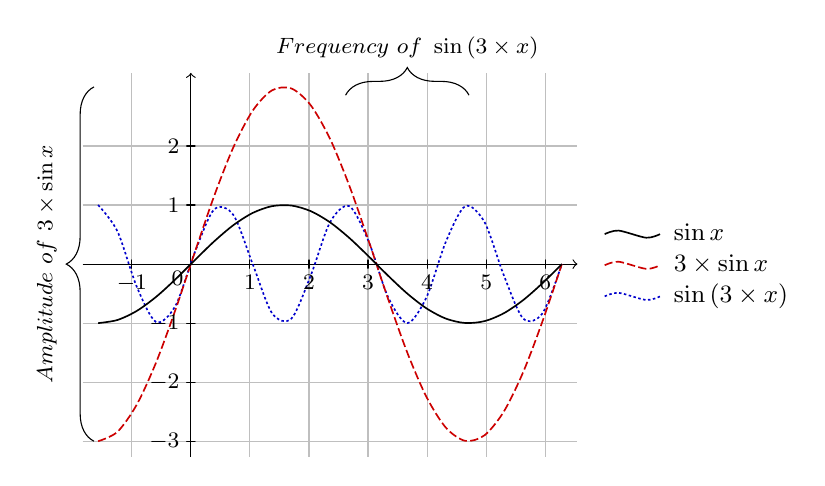
\begin{tikzpicture}[scale=.75]
			\datavisualization [
			school book axes,
			y axis=grid,
			x axis=grid,
			visualize as smooth line/.list={sina,sinb,sinc},
			style sheet=strong colors,
			style sheet=vary dashing,
			sina={label in legend={text=$\sin x$}},
			sinb={label in legend={text=$3\times{\sin x}$}},
			sinc={label in legend={text=$\sin{\left( 3 \times x \right)}$}},
			data/format=function ]
			data [set=sina] {
				var x : interval [-0.5*pi:2*pi];
				func y = sin(\value x r);
			}
			data [set=sinb] {
				var x : interval [-0.5*pi:2*pi];
				func y = 3 * sin(\value x r);
			}
			data [set=sinc] {
				var x : interval [-0.5*pi:2*pi];
				func y = sin(3 * \value x r);
			};
			\draw [decorate,decoration={brace,amplitude=10pt},xshift=-4pt,yshift=0pt]
			(-1.5,-3.0) -- (-1.5,3.0) node [black,midway,xshift=-0.6cm, rotate=90] 
			{\footnotesize $Amplitude\ of\ 3\times{\sin{x}}$};
			\draw [decorate, decoration={brace,amplitude=10pt},xshift=0pt,yshift=-4pt]
			(2.62,3.0) -- (4.71, 3.0) node [black,midway,yshift=0.6cm]
			{\footnotesize $Frequency\ of\ \sin{\left(3\times{x}\right)}$};
		\end{tikzpicture}
		
	}

	\frame{\frametitle{Where do I find more?}
		\begin{center}
			Is there something specific you want to see as an example?
			
			\href{https://texample.net/tikz/examples/}{https://texample.net/tikz/examples/}
		\end{center}
	}

	
	\section{Learning More}
	
		\frame{\frametitle{RTFM}
			\begin{center}
				\href{https://pgf-tikz.github.io/pgf/pgfmanual.pdf}{RTFM}
			\end{center}
		}
	
		\frame{\frametitle{When in doubt: Google}
			\begin{center}
			\only<1->{\TikZ has rolled into the \TeX community.\\}
			~\\
			\only<1>{~\\~\\}
			\only<2->{The community loves to help.\\}
			~\\
			\only<2>{~\\}
			\only<3>{\href{https://tex.stackexchange.com/}{https://tex.stackexchange.com/}}
			\end{center}
		}
	
		\frame{\frametitle{At your local library}
			\begin{block}{OU libraries has a \LaTeX\ expert:}
				\begin{columns}[onlytextwidth,T]
					\column{\linewidth-30mm-5mm}
						~\\~\\
						\textbf{Amanda Schilling}\\

						\faChain: \href{https://libraries.ou.edu/departments/stem-services}{Stem Services}
						
						\faPhone: (405) 325-6126
						
						\faEnvelope: \href{mailto:amanda.schilling@ou.edu}{amanda.schilling@ou.edu}
						
						~\\
						
						\textbf{Office Hours:} W/Th 8-9am in DAVIS\\
						\qquad\qquad M 6-8pm in the Learning Lab
						
					\column{30mm}
						\includegraphics[width=30mm]{amanda.jpg}
				\end{columns}
			\end{block}
		}
		
		
			\frame{\frametitle{At your local library}
			\begin{block}{OU libraries has a \LaTeX\ expert:}
				\begin{columns}[onlytextwidth,T]
					\column{\linewidth-30mm-5mm}
					~\\~\\
					\textbf{Mark Laufersweiler}\\
					
					\faChain: \href{https://libraries.ou.edu/users/mark-laufersweiler}{Research Data Specialist}
					
					\faPhone: (405) 325-3710
					
					\faEnvelope: \href{mailto:laufers@ou.edu}{laufers@ou.edu}
					
					\column{30mm}
					\includegraphics[width=30mm]{mark.jpg}
				\end{columns}
			\end{block}
		}
	
		\frame{\frametitle{Or contact me}
			\begin{block}{I'm just a \LaTeX\ junkie:}
				\begin{columns}[onlytextwidth,T]
					\column{\linewidth-30mm-5mm}
					~\\~\\
					\textbf{Wesley T. Honeycutt}\\
					
					\faChain: \href{wesleythoneycutt.com}{Personal Site}
					
					\faPhone: \emph{I have an office phone?}
					
					\faEnvelope: \href{mailto:honeycutt@ou.edu}{honeycutt@ou.edu}
					
					\faGithub: \href{https://github.com/BlueNalgene}{https://github.com/BlueNalgene}
					
					\column{30mm}
					\includegraphics[width=30mm]{wes.png}
				\end{columns}
			\end{block}
		}

\end{document}